%24.03.2018: needs github version!
\documentclass{report}
\usepackage[dvipsnames]{xcolor}
\usepackage{tikzducks}

\begin{document}
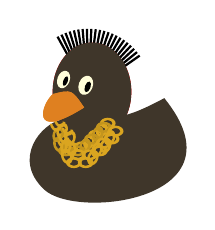
\begin{tikzpicture}

\fill[red]
(0.90,1.50) ellipse (0.50 and 0.625);
\foreach \x in {0,4,...,42} %{35,39,...,120}
 {\draw[thick,](0.85,1.50)--++(\x+35:0.8cm);}
\foreach \x in {2,6,...,42} %{35,39,...,120}
 {\draw[thick](0.85,1.50)--++(\x+77:0.8cm);}
 \duck[body=Tan!30!black,,grumpy]
\begin{scope}[yshift=1.0cm,xshift=-1mm]
%\fill[Goldenrod] (1.5,0.25) circle (0.3);
	\fill[Goldenrod, even odd rule] (1.2,0.1) ellipse (0.10 and 0.07) (1.2,0.1) ellipse (0.06 and 0.04) (1.05,-0.05) ellipse (0.10 and 0.07) (1.05,-0.05) ellipse (0.06 and 0.04) (0.87,-0.2) ellipse (0.10 and 0.07) (0.87,-0.2) ellipse (0.06 and 0.04);
	\fill[Goldenrod, even odd rule] (0.72,-0.2) ellipse (0.10 and 0.07) (0.72,-0.2) ellipse (0.06 and 0.04);	
	\fill[Goldenrod,even odd rule,rotate=70](0.4,-1.05) ellipse (0.1 and 0.07) (0.4,-1.05) ellipse (0.06 and 0.04) (0.2,-0.95) ellipse (0.1 and 0.07) (0.2,-0.95) ellipse (0.06 and 0.04) (0.22,-0.58) ellipse (0.1 and 0.07) (0.22,-0.58) ellipse (0.06 and 0.04);
	\fill[Goldenrod,even odd rule,rotate=110](-0.33,-0.55) ellipse (0.1 and 0.07) (-0.33,-0.55) ellipse (0.06 and 0.04);	
	\begin{scope}
		\clip[rotate=-12] (0.45,0.15) rectangle (0.63,0.25);	
		\fill[Goldenrod,even odd rule,rotate=110](-0.07,-0.6) ellipse (0.1 and 0.07) (-0.07,-0.6) ellipse (0.06 and 0.04);	
	\end{scope}
\end{scope}
\begin{scope}[yshift=0.95cm,xshift=-1.5mm]
%\fill[Goldenrod] (1.5,0.25) circle (0.3);
	\fill[Goldenrod!90!black, even odd rule] (1.2,0.1) ellipse (0.10 and 0.07) (1.2,0.1) ellipse (0.06 and 0.04) (1.05,-0.05) ellipse (0.10 and 0.07) (1.05,-0.05) ellipse (0.06 and 0.04) (0.87,-0.2) ellipse (0.10 and 0.07) (0.87,-0.2) ellipse (0.06 and 0.04);
	\fill[Goldenrod!90!black, even odd rule] (0.72,-0.2) ellipse (0.10 and 0.07) (0.72,-0.2) ellipse (0.06 and 0.04);	
	\fill[Goldenrod!90!black,even odd rule,rotate=70](0.4,-1.05) ellipse (0.1 and 0.07) (0.4,-1.05) ellipse (0.06 and 0.04) (0.2,-0.95) ellipse (0.1 and 0.07) (0.2,-0.95) ellipse (0.06 and 0.04) (0.22,-0.58) ellipse (0.1 and 0.07) (0.22,-0.58) ellipse (0.06 and 0.04);
	\fill[Goldenrod!90!black,even odd rule,rotate=110](-0.33,-0.55) ellipse (0.1 and 0.07) (-0.33,-0.55) ellipse (0.06 and 0.04);	
	\begin{scope}
		\clip[rotate=-12] (0.45,0.15) rectangle (0.63,0.25);	
		\fill[Goldenrod,even odd rule,rotate=110](-0.07,-0.6) ellipse (0.1 and 0.07) (-0.07,-0.6) ellipse (0.06 and 0.04);	
	\end{scope}
\end{scope}
\begin{scope}[yshift=0.90cm,xshift=0mm]
%\fill[Goldenrod] (1.5,0.25) circle (0.3);
	\fill[Goldenrod, even odd rule] (1.2,0.1) ellipse (0.10 and 0.07) (1.2,0.1) ellipse (0.06 and 0.04) (1.05,-0.05) ellipse (0.10 and 0.07) (1.05,-0.05) ellipse (0.06 and 0.04) (0.87,-0.2) ellipse (0.10 and 0.07) (0.87,-0.2) ellipse (0.06 and 0.04);
	\fill[Goldenrod, even odd rule] (0.72,-0.2) ellipse (0.10 and 0.07) (0.72,-0.2) ellipse (0.06 and 0.04);	
	\fill[Goldenrod,even odd rule,rotate=70](0.4,-1.05) ellipse (0.1 and 0.07) (0.4,-1.05) ellipse (0.06 and 0.04) (0.2,-0.95) ellipse (0.1 and 0.07) (0.2,-0.95) ellipse (0.06 and 0.04) (0.22,-0.58) ellipse (0.1 and 0.07) (0.22,-0.58) ellipse (0.06 and 0.04);
	\fill[Goldenrod,even odd rule,rotate=110](-0.33,-0.55) ellipse (0.1 and 0.07) (-0.33,-0.55) ellipse (0.06 and 0.04);	
	\begin{scope}
		\clip[rotate=-12] (0.45,0.15) rectangle (0.63,0.25);	
		\fill[Goldenrod,even odd rule,rotate=110](-0.07,-0.6) ellipse (0.1 and 0.07) (-0.07,-0.6) ellipse (0.06 and 0.04);	
	\end{scope}
\end{scope}
\begin{scope}[yshift=0.80cm,xshift=-0.5mm]
%\fill[Goldenrod] (1.5,0.25) circle (0.3);
	\fill[Goldenrod, even odd rule] (1.2,0.1) ellipse (0.10 and 0.07) (1.2,0.1) ellipse (0.06 and 0.04) (1.05,-0.05) ellipse (0.10 and 0.07) (1.05,-0.05) ellipse (0.06 and 0.04) (0.87,-0.2) ellipse (0.10 and 0.07) (0.87,-0.2) ellipse (0.06 and 0.04);
	\fill[Goldenrod, even odd rule] (0.72,-0.2) ellipse (0.10 and 0.07) (0.72,-0.2) ellipse (0.06 and 0.04);	
	\fill[Goldenrod,even odd rule,rotate=70](0.4,-1.05) ellipse (0.1 and 0.07) (0.4,-1.05) ellipse (0.06 and 0.04) (0.2,-0.95) ellipse (0.1 and 0.07) (0.2,-0.95) ellipse (0.06 and 0.04) (0.22,-0.58) ellipse (0.1 and 0.07) (0.22,-0.58) ellipse (0.06 and 0.04);
	\fill[Goldenrod,even odd rule,rotate=110](-0.33,-0.55) ellipse (0.1 and 0.07) (-0.33,-0.55) ellipse (0.06 and 0.04);	
	\begin{scope}
		\clip[rotate=-12] (0.45,0.15) rectangle (0.63,0.25);	
		\fill[Goldenrod,even odd rule,rotate=110](-0.07,-0.6) ellipse (0.1 and 0.07) (-0.07,-0.6) ellipse (0.06 and 0.04);	
	\end{scope}
\end{scope}


\fill[orange!50!brown]\duckpathgrumpybill;

\end{tikzpicture}

%needs github version of tikzducks!!!

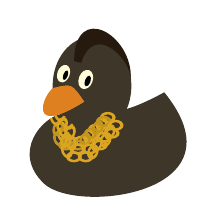
\begin{tikzpicture}
\duck[mohican=black!80!brown,body=Tan!30!black,,grumpy];
\begin{scope}[yshift=1.0cm,xshift=-1mm]
%\fill[Goldenrod] (1.5,0.25) circle (0.3);
	\fill[Goldenrod, even odd rule] (1.2,0.1) ellipse (0.10 and 0.07) (1.2,0.1) ellipse (0.06 and 0.04) (1.05,-0.05) ellipse (0.10 and 0.07) (1.05,-0.05) ellipse (0.06 and 0.04) (0.87,-0.2) ellipse (0.10 and 0.07) (0.87,-0.2) ellipse (0.06 and 0.04);
	\fill[Goldenrod, even odd rule] (0.72,-0.2) ellipse (0.10 and 0.07) (0.72,-0.2) ellipse (0.06 and 0.04);	
	\fill[Goldenrod,even odd rule,rotate=70](0.4,-1.05) ellipse (0.1 and 0.07) (0.4,-1.05) ellipse (0.06 and 0.04) (0.2,-0.95) ellipse (0.1 and 0.07) (0.2,-0.95) ellipse (0.06 and 0.04) (0.22,-0.58) ellipse (0.1 and 0.07) (0.22,-0.58) ellipse (0.06 and 0.04);
	\fill[Goldenrod,even odd rule,rotate=110](-0.33,-0.55) ellipse (0.1 and 0.07) (-0.33,-0.55) ellipse (0.06 and 0.04);	
	\begin{scope}
		\clip[rotate=-12] (0.45,0.15) rectangle (0.63,0.25);	
		\fill[Goldenrod,even odd rule,rotate=110](-0.07,-0.6) ellipse (0.1 and 0.07) (-0.07,-0.6) ellipse (0.06 and 0.04);	
	\end{scope}
\end{scope}
\begin{scope}[yshift=0.95cm,xshift=-1.5mm]
%\fill[Goldenrod] (1.5,0.25) circle (0.3);
	\fill[Goldenrod!90!black, even odd rule] (1.2,0.1) ellipse (0.10 and 0.07) (1.2,0.1) ellipse (0.06 and 0.04) (1.05,-0.05) ellipse (0.10 and 0.07) (1.05,-0.05) ellipse (0.06 and 0.04) (0.87,-0.2) ellipse (0.10 and 0.07) (0.87,-0.2) ellipse (0.06 and 0.04);
	\fill[Goldenrod!90!black, even odd rule] (0.72,-0.2) ellipse (0.10 and 0.07) (0.72,-0.2) ellipse (0.06 and 0.04);	
	\fill[Goldenrod!90!black,even odd rule,rotate=70](0.4,-1.05) ellipse (0.1 and 0.07) (0.4,-1.05) ellipse (0.06 and 0.04) (0.2,-0.95) ellipse (0.1 and 0.07) (0.2,-0.95) ellipse (0.06 and 0.04) (0.22,-0.58) ellipse (0.1 and 0.07) (0.22,-0.58) ellipse (0.06 and 0.04);
	\fill[Goldenrod!90!black,even odd rule,rotate=110](-0.33,-0.55) ellipse (0.1 and 0.07) (-0.33,-0.55) ellipse (0.06 and 0.04);	
	\begin{scope}
		\clip[rotate=-12] (0.45,0.15) rectangle (0.63,0.25);	
		\fill[Goldenrod,even odd rule,rotate=110](-0.07,-0.6) ellipse (0.1 and 0.07) (-0.07,-0.6) ellipse (0.06 and 0.04);	
	\end{scope}
\end{scope}
\begin{scope}[yshift=0.90cm,xshift=0mm]
%\fill[Goldenrod] (1.5,0.25) circle (0.3);
	\fill[Goldenrod, even odd rule] (1.2,0.1) ellipse (0.10 and 0.07) (1.2,0.1) ellipse (0.06 and 0.04) (1.05,-0.05) ellipse (0.10 and 0.07) (1.05,-0.05) ellipse (0.06 and 0.04) (0.87,-0.2) ellipse (0.10 and 0.07) (0.87,-0.2) ellipse (0.06 and 0.04);
	\fill[Goldenrod, even odd rule] (0.72,-0.2) ellipse (0.10 and 0.07) (0.72,-0.2) ellipse (0.06 and 0.04);	
	\fill[Goldenrod,even odd rule,rotate=70](0.4,-1.05) ellipse (0.1 and 0.07) (0.4,-1.05) ellipse (0.06 and 0.04) (0.2,-0.95) ellipse (0.1 and 0.07) (0.2,-0.95) ellipse (0.06 and 0.04) (0.22,-0.58) ellipse (0.1 and 0.07) (0.22,-0.58) ellipse (0.06 and 0.04);
	\fill[Goldenrod,even odd rule,rotate=110](-0.33,-0.55) ellipse (0.1 and 0.07) (-0.33,-0.55) ellipse (0.06 and 0.04);	
	\begin{scope}
		\clip[rotate=-12] (0.45,0.15) rectangle (0.63,0.25);	
		\fill[Goldenrod,even odd rule,rotate=110](-0.07,-0.6) ellipse (0.1 and 0.07) (-0.07,-0.6) ellipse (0.06 and 0.04);	
	\end{scope}
\end{scope}
\begin{scope}[yshift=0.80cm,xshift=-0.5mm]
%\fill[Goldenrod] (1.5,0.25) circle (0.3);
	\fill[Goldenrod, even odd rule] (1.2,0.1) ellipse (0.10 and 0.07) (1.2,0.1) ellipse (0.06 and 0.04) (1.05,-0.05) ellipse (0.10 and 0.07) (1.05,-0.05) ellipse (0.06 and 0.04) (0.87,-0.2) ellipse (0.10 and 0.07) (0.87,-0.2) ellipse (0.06 and 0.04);
	\fill[Goldenrod, even odd rule] (0.72,-0.2) ellipse (0.10 and 0.07) (0.72,-0.2) ellipse (0.06 and 0.04);	
	\fill[Goldenrod,even odd rule,rotate=70](0.4,-1.05) ellipse (0.1 and 0.07) (0.4,-1.05) ellipse (0.06 and 0.04) (0.2,-0.95) ellipse (0.1 and 0.07) (0.2,-0.95) ellipse (0.06 and 0.04) (0.22,-0.58) ellipse (0.1 and 0.07) (0.22,-0.58) ellipse (0.06 and 0.04);
	\fill[Goldenrod,even odd rule,rotate=110](-0.33,-0.55) ellipse (0.1 and 0.07) (-0.33,-0.55) ellipse (0.06 and 0.04);	
	\begin{scope}
		\clip[rotate=-12] (0.45,0.15) rectangle (0.63,0.25);	
		\fill[Goldenrod,even odd rule,rotate=110](-0.07,-0.6) ellipse (0.1 and 0.07) (-0.07,-0.6) ellipse (0.06 and 0.04);	
	\end{scope}
\end{scope}
\fill[orange!50!brown]\duckpathgrumpybill;
\end{tikzpicture}

\end{document}